\documentclass{beamer}
\usepackage[utf8]{inputenc}

\usetheme{Madrid}
\usecolortheme{default}
\usepackage{amsmath,amssymb,amsfonts,amsthm}
\usepackage{txfonts}
\usepackage{tkz-euclide}
\usepackage{listings}
\usepackage{adjustbox}
\usepackage{array}
\usepackage{tabularx}
\usepackage{gvv}
\usepackage{lmodern}
\usepackage{circuitikz}
\usepackage{tikz}
\usepackage{graphicx}

\setbeamertemplate{page number in head/foot}[totalframenumber]

\usepackage{tcolorbox}
\tcbuselibrary{minted,breakable,xparse,skins}



\definecolor{bg}{gray}{0.95}
\DeclareTCBListing{mintedbox}{O{}m!O{}}{%
  breakable=true,
  listing engine=minted,
  listing only,
  minted language=#2,
  minted style=default,
  minted options={%
    linenos,
    gobble=0,
    breaklines=true,
    breakafter=,,
    fontsize=\small,
    numbersep=8pt,
    #1},
  boxsep=0pt,
  left skip=0pt,
  right skip=0pt,
  left=25pt,
  right=0pt,
  top=3pt,
  bottom=3pt,
  arc=5pt,
  leftrule=0pt,
  rightrule=0pt,
  bottomrule=2pt,

  colback=bg,
  colframe=orange!70,
  enhanced,
  overlay={%
    \begin{tcbclipinterior}
    \fill[orange!20!white] (frame.south west) rectangle ([xshift=20pt]frame.north west);
    \end{tcbclipinterior}},
  #3,
}
\lstset{
    language=C,
    basicstyle=\ttfamily\small,
    keywordstyle=\color{blue},
    stringstyle=\color{orange},
    commentstyle=\color{green!60!black},
    numbers=left,
    numberstyle=\tiny\color{gray},
    breaklines=true,
    showstringspaces=false,
}
%------------------------------------------------------------
%This block of code defines the information to appear in the
%Title page
\title %optional
{4.2.15}
\date{September  2025}
%\subtitle{A short story}

\author % (optional)
{BEERAM MADHURI - EE25BTECH11012}



\begin{document}


\frame{\titlepage}
\begin{frame}{Question}
Find the direction and normal vectors of $y=2x$.

\end{frame}
 
\begin{frame}{given data}
 
Line equation is $y=2x$
   
\end{frame}

\begin{frame}{solution}
    \frametitle{finding direction and normal vectors of $y=2x$}
The line can be written as:
\begin{align}
-2x + 1y = 0
\end{align}
This equation can be expressed in terms of matrices as:
\begin{align}
\vec{n}^\top \vec{x} = c\\
\vec{n}^\top = \begin{pmatrix} -2 & 1 \end{pmatrix}\\
\vec{x} = \begin{pmatrix} x \\ y \end{pmatrix}\\
c = 0
\end{align}
where $\vec{n}$ is normal vector of the given line.

The direction vector is:
\begin{align}
\vec{m} = \begin{pmatrix} 1 \\ 2 \end{pmatrix}.
\end{align}
\end{frame}
\begin{frame}
This is true because, if the direction vector is represented as
\begin{align}
\vec{m} = \begin{pmatrix} 1 \\ m \end{pmatrix}
\end{align}
then the normal vector can be expressed as
\begin{align}
  \vec{n} = \begin{pmatrix} -m \\ 1 \end{pmatrix} \\
  \vec{n}^\top \vec{m} =0\\
   \begin{pmatrix} -2 & 1 \end{pmatrix}\begin{pmatrix} 1 \\ 2 \end{pmatrix}=0
\end{align}
Hence, normal vector $\vec{n} = \begin{pmatrix} -2 \\ 1 \end{pmatrix}$ and direction vector  $\vec{m} = \begin{pmatrix} 1 \\ 2 \end{pmatrix}$.

\end{frame}


\begin{frame}[fragile]
    \frametitle{Python Code}
    \begin{lstlisting}
 import matplotlib.pyplot as plt
import numpy as np

# --- 1. Vector Calculation ---
# The equation of the line is y = 2x.
# The standard form is Ax + By + C = 0, which is 2x - y = 0.
A = 2
B = -1

# The normal vector is <A, B>. It's perpendicular to the line.
normal_vector = np.array([A, B])

\end{lstlisting}
\end{frame}

\begin{frame}[fragile]
    \frametitle{Python Code}

    \begin{lstlisting}
# The direction vector is <-B, A>. It's parallel to the line.
direction_vector = np.array([-B, A])

print(f"Line Equation: y = 2x")
print("-" * 25)
print(f"Direction Vector: {tuple(direction_vector)}")
print(f"Normal Vector:    {tuple(normal_vector)}")

    \end{lstlisting}
\end{frame}

\begin{frame}[fragile]
    \frametitle{Python Code}

    \begin{lstlisting}
# Create a figure and a set of subplots
fig, ax = plt.subplots(figsize=(8, 8))

# Generate x values for our line
x_vals = np.linspace(-2.5, 2.5, 100)
# Calculate the corresponding y values for the line y = 2x
y_vals = 2 * x_vals

# Plot the main line
ax.plot(x_vals, y_vals, label='Line: y = 2x', color='blue', zorder=1)
    \end{lstlisting}
\end{frame}

\begin{frame}[fragile]
    \frametitle{Python Code}

    \begin{lstlisting}
# Plot the vectors as arrows starting from the origin (0,0)
# The 'quiver' function is used to plot arrows.

# Plot the Direction Vector (green)
ax.quiver(0, 0, direction_vector[0], direction_vector[1],
          angles='xy', scale_units='xy', scale=1,
          color='green', label=f'Direction Vector: {tuple(direction_vector)}', zorder=2)

# Plot the Normal Vector (red)
ax.quiver(0, 0, normal_vector[0], normal_vector[1],
          angles='xy', scale_units='xy', scale=1,
          color='red', label=f'Normal Vector: {tuple(normal_vector)}', zorder=2)
\end{lstlisting}
\end{frame}

 
\begin{frame}[fragile]
    \frametitle{Python Code}

    \begin{lstlisting}
# Set the aspect ratio of the plot to be equal, so 90-degree angles look correct
ax.set_aspect('equal')

# Set the limits for the x and y axes
ax.set_xlim(-4, 4)
ax.set_ylim(-4, 4)

# Move the x and y axes to the center of the plot
ax.spines['left'].set_position('zero')
ax.spines['bottom'].set_position('zero')
ax.spines['right'].set_color('none')
ax.spines['top'].set_color('none')
\end{lstlisting}
\end{frame}
\begin{frame}[fragile]
    \frametitle{Python Code}

    \begin{lstlisting}
# Add a grid for better readability
ax.grid(True, linestyle='--')

# Add a title and a legend
ax.set_title("Line y=2x with its Direction and Normal Vectors", fontsize=14)
ax.legend(loc='upper left')

# Display the plot
plt.show()
\end{lstlisting}
\end{frame}

\begin{frame}[fragile]
\frametitle{C Code}
\begin{lstlisting}
#include <stdio.h>
// A simple structure to represent a 2D vector
typedef struct {
    float x;
    float y;
} Vector2D;
int main() {
    // Equation of the line: y = 2x
    // General form: 2x - 1y + 0 = 0
    // So, A = 2 and B = -1
\end{lstlisting}
\end{frame}

\begin{frame}[fragile]
\frametitle{C Code}
\begin{lstlisting}
    float A = 2.0f;
    float B = -1.0f;
    // Declare vectors
    Vector2D normal_vector;
    Vector2D direction_vector;
    // For a line Ax + By + C = 0:
    // A normal vector is given by n = (A, B)
    normal_vector.x = A;
    normal_vector.y = B;
\end{lstlisting}
\end{frame}

\begin{frame}[fragile]
\frametitle{C Code}
\begin{lstlisting}
    // A direction vector is perpendicular to the normal vector.
    // It can be found as d = (-B, A) or (B, -A)
    direction_vector.x = -B;
    direction_vector.y = A;
    printf("For the line y = 2x (or 2x - y = 0):\n");
    printf("----------------------------------------\n");
    printf("Calculated Normal Vector   (A, B)  : <%.1f, %.1f>\n", normal_vector.x, normal_vector.y);
    printf("Calculated Direction Vector (-B, A): <%.1f, %.1f>\n", direction_vector.x, direction_vector.y);
    return 0;
}
\end{lstlisting}
\end{frame}


\begin{frame}[fragile]
\frametitle{Python and C Code}
\begin{lstlisting}
import ctypes
import platform
# --- 1. Define a Python class that mirrors the C struct ---
class Vector2D(ctypes.Structure):
    fields = [("x", ctypes.c_float),
                ("y", ctypes.c_float)]
\end{lstlisting}
\end{frame}


\begin{frame}[fragile]
\frametitle{Python and C Code}
\begin{lstlisting}
# --- 2. Load the shared library ---
if platform.system() == "Windows":
    lib_path = "./libline.dll"
else:
    lib_path = "./libline.so"

try:
    lib = ctypes.CDLL(lib_path)
except OSError as e:
    print(f"Error loading library: {e}")
    print("Have you compiled line_vectors.c?")
    exit()
\end{lstlisting}
\end{frame}


\begin{frame}[fragile]
\frametitle{Python and C Code}
\begin{lstlisting}
# --- 3. Define the function signature ---
lib.get_line_vectors.argtypes = [
    ctypes.c_float,            # A
    ctypes.c_float,            # B
    ctypes.POINTER(Vector2D),  # normal_out (output)
    ctypes.POINTER(Vector2D)   # direction_out (output)
]
lib.get_line_vectors.restype = None
\end{lstlisting}
\end{frame}


\begin{frame}[fragile]
\frametitle{Python and C Code}
\begin{lstlisting}
# --- 4. Prepare data and call the C function ---
# Hardcoded input values for the line 2x - y = 0
A = 2.0
B = -1.0

# Create empty instances of our Vector2D class for the output
normal_vector = Vector2D()
direction_vector = Vector2D()
\end{lstlisting}
\end{frame}

\begin{frame}[fragile]
\frametitle{Python and C Code}
\begin{lstlisting}
# Call the C function with the hardcoded inputs
lib.get_line_vectors(A, B, ctypes.byref(normal_vector), ctypes.byref(direction_vector))
# --- 5. Print the results ---
print("For the line y = 2x (or 2x - y = 0):")
print("----------------------------------------")
print(f"Calculated Normal Vector   (A, B)  : <{normal_vector.x:.1f}, {normal_vector.y:.1f}>")
print(f"Calculated Direction Vector (-B, A): <{direction_vector.x:.1f}, {direction_vector.y:.1f}>")
\end{lstlisting}
\end{frame}
\begin{frame}
\begin{figure}
    \centering
    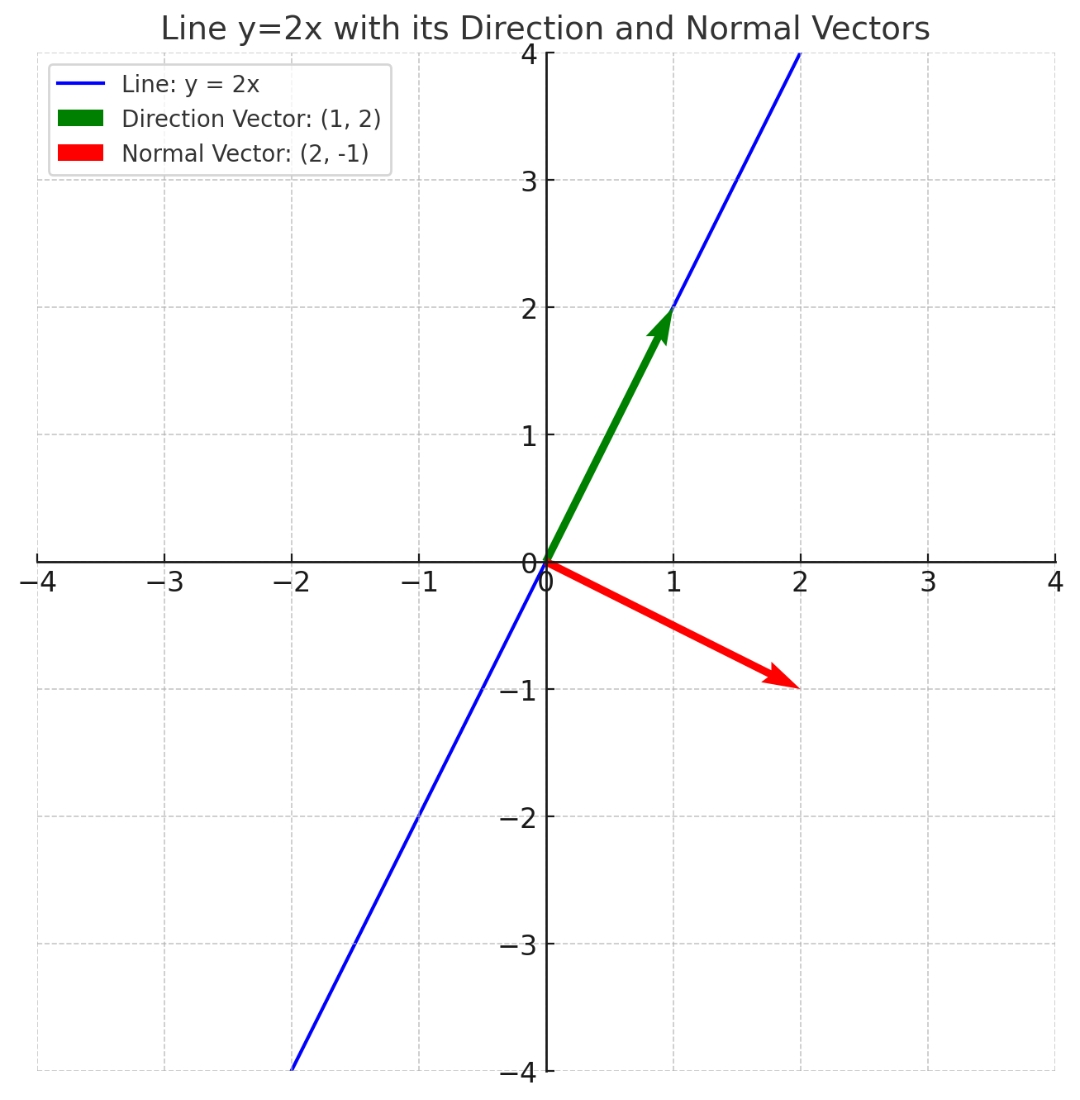
\includegraphics[width=0.75\columnwidth]{graph-6.jpg}
    \caption{Plot}
    \label{fig:placeholder}
\end{figure}
\end{frame}

\end{document}